\documentclass[10pt]{article}
\usepackage[margin=.65in]{geometry}
\usepackage{graphicx,booktabs,hyperref,amsmath,amssymb,array}
\hypersetup{colorlinks=true,urlcolor=blue}
\setlength{\parindent}{0pt}
\setlength{\parskip}{5pt}
\begin{document}
\begin{center}
{\Large Relation yield on a quadratic twist}\\[4pt]
{\large Exact count/rank theorems and a conditional IC cost comparison}\\[4pt]
24 October 2026 $\cdot$ \texttt{yield-20261024} $\cdot$ PR \#2381
\end{center}
\textbf{Request.} Relate twist and main-curve relation yield in Lean, and show
how higher yield and lower degree of regularity could make index calculus faster.
The checked result distinguishes matched transport, different rational groups,
useful independent rows and a conditional solver-cost model. Neither a yield
improvement nor lower regularity is assumed to follow merely from twisting.

For an indexed finite factor base $B=(B_i)$ and a finite set $C$ of integer
coefficient vectors, define
\[
R(B,C)=\{c\in C:\textstyle\sum_i[c_i]B_i=O\}.
\]
For every injective additive homomorphism $f$, Lean proves
\[
\boxed{R(f(B),C)=R(B,C).}
\]
The accepted coefficient sets, normalized raw yields, coefficient-row spans
and ranks over every chosen field are identical. The same useful-row predicate
gives identical useful yield. The theorem is instantiated on the actual map
$\psi:E_d(k)\to E(K)$, $(X,Y)\mapsto(X/d,Y/(du))$, $u^2=d$, $d\ne0$,
for an elliptic short model. The target is the twist image inside $E(K)$;
no equality with the different rational group $E(k)$ is assumed.

\begin{center}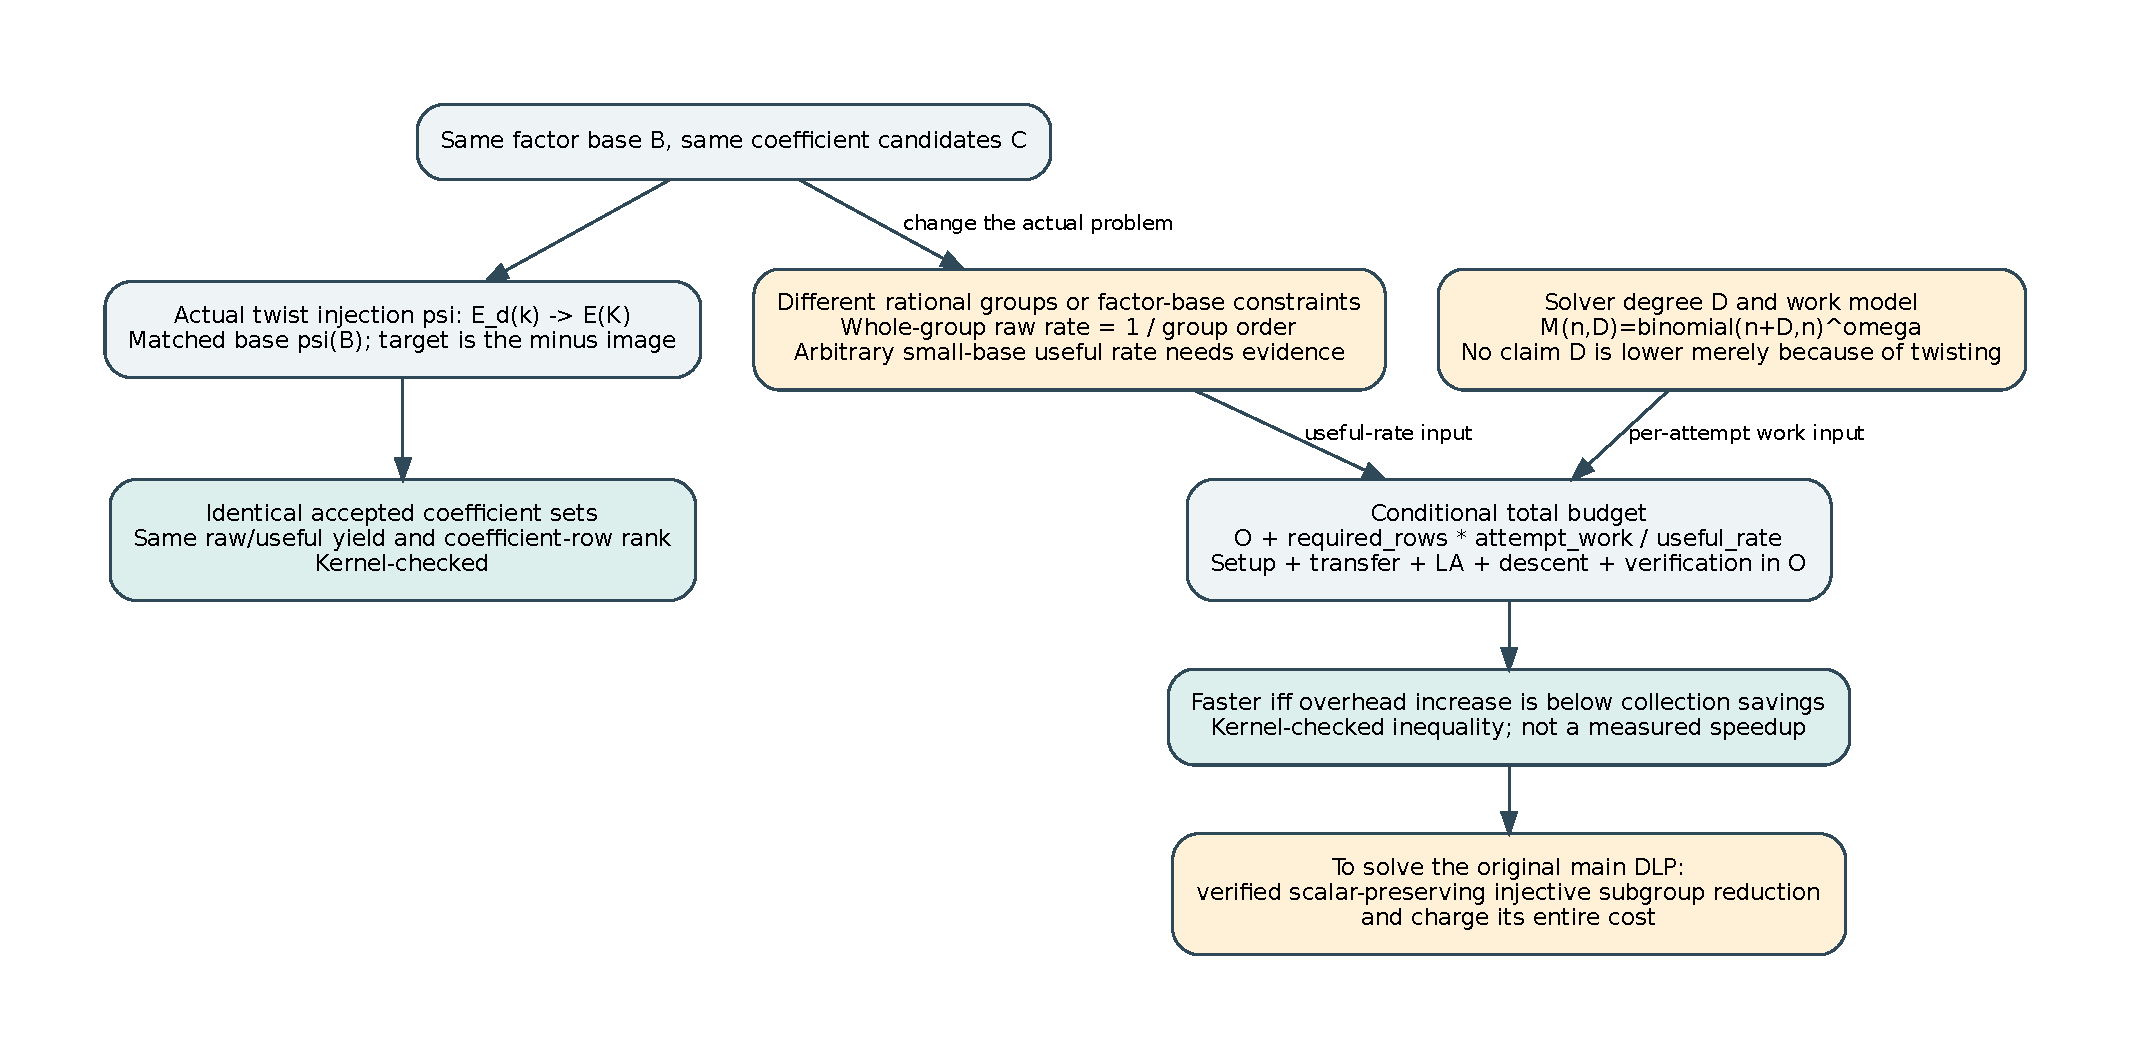
\includegraphics[height=4.8in,width=\linewidth,keepaspectratio]{bridge.pdf}\end{center}
\small Green boxes identify kernel-checked results; amber boxes identify
inputs/conditions still needed for an actual solver advantage.\normalsize

\newpage
\begin{center}{\Large A yield relationship and a cost threshold}\end{center}
\textbf{Uniform whole-group yield.} In a finite group of order $N$, every
ordered prefix of length $m$ has exactly one final point completing its sum to
zero. Lean constructs the equivalence and proves
\[
\#R=N^m,\quad \#C=N^{m+1},\quad p_{\rm raw}=1/N.
\]
For main/twist rational groups of actual orders $N,N_t$ and the same tuple length,
\[
\boxed{p_{\rm raw,T}/p_{\rm raw,E}=N/N_t.}
\]
Thus a smaller twist group has higher raw whole-group yield. This concerns
uniform sampling from the entire groups, including the $m=0$ case. It is not
a distribution theorem for a small IC factor base or for independent rows.
The formal statements count zero-sum tuples and do not add a general elliptic
point-counting theorem. They use the actual group orders supplied.

\textbf{Useful work accounting.} Let $p_X>0$ be useful independent-row yield,
$c_X$ work per attempt and $m_X$ the required number of useful rows. Charge
setup, subgroup transfer, linear algebra, descent and verification in $O_X$.
Define the conditional budget
\[
\mathcal C_X=O_X+m_X\frac{c_X}{p_X}.
\]
For a finite batch with attempts $A>0$, useful rows $U>0$ and work $W$, Lean
proves $(W/A)/(U/A)=W/U$. Extrapolation to later rank states is an additional
assumption. This is not a proved stochastic completion-time model.

Lean proves the exact overhead threshold, including different row requirements:
\[
\boxed{\mathcal C_T<\mathcal C_E\ \Longleftrightarrow\
O_T-O_E<m_Ec_E/p_E-m_Tc_T/p_T.}
\]
For common $m>0$, $O_T\le O_E$, $p_T>p_E>0$, and $c_T\le c_E$ with $c_E>0$,
the twist budget is strictly smaller. Strictly lower attempt work also suffices
when useful yield does not decrease.

\textbf{Degree model.} Define the explicit dense monomial model
\[
M(n,D,\omega)=\binom{n+D}{n}^{\omega}.
\]
Here $n,D,\omega$ are natural numbers; $\omega=3$ is an allowed dense work model.
Lean proves monotonicity in $D$, strict for $n>0$ and $\omega>0$.
At fixed $n,\omega$, lower $D$ and higher useful yield therefore meet the
sufficient cost conditions. Strictly lower $D$ can also suffice at equal yield.
The core declarations are \texttt{faster\_of\_yield\_and\_degree} and
\texttt{faster\_of\_strict\_degree}.

\textbf{The missing regularity bridge.} $D$ is a supplied relevant solver-degree
parameter. These theorems do not define an actual ideal's regularity, prove that
a curve system has this $D$, prove a regularity-to-solving-degree bound, or prove
this dense formula describes F4/F5 work. Actual equations, rationality/field
constraints, variable count, order, sparsity and coefficient costs must justify
that connection. Lower $D$ alone does not compare systems with different shapes.

\newpage
\begin{center}{\Large Control: more raw relations can give no useful rows}\end{center}
The existing registered F5 models are
\begin{align*}
E &: y^2=x^3+x+1, &P&=(0,1), &\#E&=9,\\
E_d &: Y^2=X^3+4X+3, &U&=(2,2), &\#E_d&=3.
\end{align*}
Here $d=2$ and $E_d$ is the monic twist. Their model identities are
\texttt{icv1-fp3-tm3-37e7e540} and \texttt{icv1-fp3-t3-cec99b6b}.
The original model records have no selected EC1 subgroup representations;
none is invented here. Actual nonsingular points, $[9]P=O$, $[3]P\ne O$,
$[3]U=O$ and $U\ne O$ are kernel-checked.

For the same nine scalar candidates $n=0,\ldots,8$, Lean checks one zero
$[n]P=O$ on the main point and three zeros $[n]U=O$ on the twist point.
But every twist zero satisfies $n\bmod3=0$. Thus there are
\textbf{zero nonzero coefficient rows modulo3} for that order3 logarithm.
The raw gain is not a rank-information gain. The compared point orders differ;
this is not a comparison of equal-size prime-order DLP instances.

\begin{center}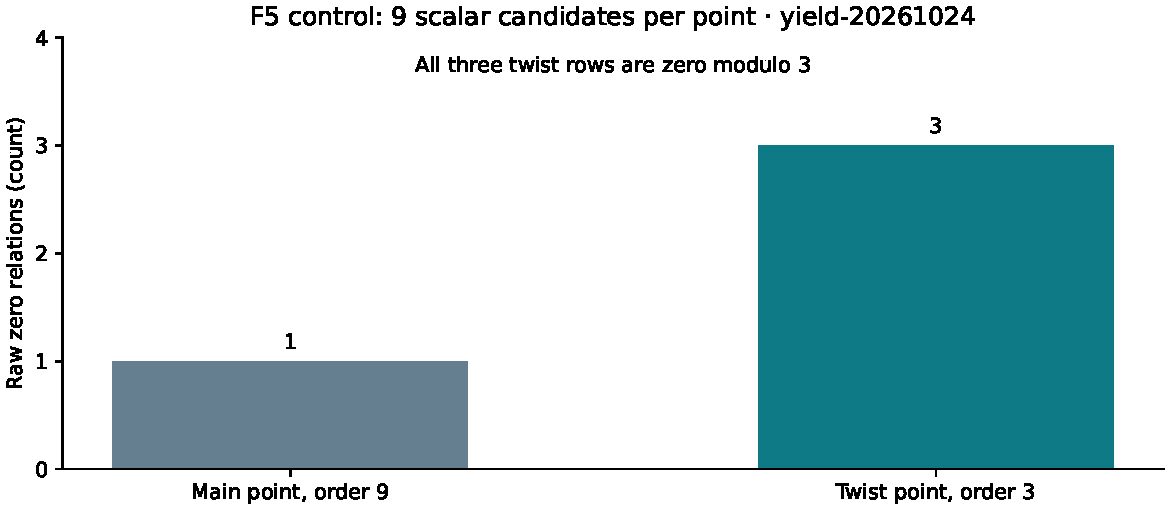
\includegraphics[width=.95\linewidth]{raw-yield.pdf}\end{center}
\small Exact kernel-certified integer counts from \texttt{YieldFixture},
\texttt{yield-20261024}; nine candidates per point. No timing, sampling interval
or performance claim. Python only lays out these recorded values.\normalsize

\textbf{Synthetic budget controls.} Separate from the F5 curves, the checked
model admits a gain for $n=2$, $\omega=3$, $D_T=2$, $D_E=3$,
$p_T=1/5$, $p_E=1/10$, $m=10$, $O_T=5000$ and $O_E=0$.
The same per-attempt/rate parameters lose for $m=1$ and $O_T=100000$.
These are explicitly synthetic rational-budget examples, not costs measured
on either curve. They check both sides of the overhead criterion.

\textbf{Helping the original DLP.} A cheaper twist problem is useful for the
main problem only after a verified scalar-preserving injective subgroup
reduction is supplied. \texttt{scalar\_solution\_iff} proves its exact
scalar-transport implication. The known twist map into $E(K)$ does not by itself
give this reduction between $E(k)$ and $E_d(k)$; existing eigenspace and coprime
order obstructions remain. The entire transfer cost belongs in $O_T$.

\newpage
\begin{center}{\Large Proof map, validation and scope}\end{center}
\begin{tabular}{p{.37\linewidth}p{.58\linewidth}}
\toprule
Claim & Checked declaration(s)\\\midrule
Accepted coefficient-set equality & \texttt{RelationYield.relationRows\_transport}\\
Actual coefficient span/rank & \texttt{rowSpace\_transport}, \texttt{rowRank\_transport}\\
Actual twist count/rank instantiation & \texttt{twist\_relationRows}, \texttt{twist\_rawYield}, \texttt{twist\_rowRank}\\
Whole-group count/yield/ratio & \texttt{full\_relation\_count},\newline \texttt{full\_factor\_base\_yield}, \texttt{full\_yield\_ratio}\\
Useful batch normalization & \texttt{RelationCost.batch\_normalization}\\
Overhead and degree implications & \texttt{overhead\_threshold\_general}, \texttt{faster\_of\_yield\_and\_degree}, \texttt{faster\_of\_strict\_degree}\\
Actual pipeline comparison & \texttt{actual\_faster\_of\_bounds}, with independently justified work bounds\\
Finite raw-count control & \texttt{YieldFixture}, eleven named statements\\\bottomrule
\end{tabular}

The new modules add \textbf{38 named theorems}. The unchanged scoped repository
gate passes \textbf{106 named research theorems / 127 audited declarations},
including21 generated helpers, in ten modules, with zero failing or extra
trusted native axioms. Only \texttt{propext}, \texttt{Classical.choice} and
\texttt{Quot.sound} occur. Lean4.34.1 and the following Mathlib commit remain pinned:
\par\texttt{d13f23b723b8a846827a245b89c10fc7d3f11612}\par
No external \texttt{lean4checker} replay is claimed; the tool is unavailable.

The polynomial part of clearing the cost denominators has source-bound
certificate \texttt{IDC1h1fac46ceb41801ac}, with32+16 native replay points,
an arithmetic false-plus-one counterexample and rejected false Lean hash.
It does not certify actual yield, regularity or runtime. The native harness
replays exact bytes and22 backend tests. Lean separately checks positivity,
counts, ranks and inequalities. No Python research execution is introduced.

\textbf{Reproduce.}
\begin{verbatim}
tools/lean/proof-gate.sh --out /tmp/twist-yield-proof \
  research/quadratic_twist_evidence_20261021/lean
bash research/quadratic_twist_evidence_20261021/run-yield.sh \
  /tmp/twist-yield-fresh
\end{verbatim}
Protocol \texttt{65bea0a7ef8dad84453c30d61bdc9efedee28354} preceded execution.
The source-linked Markdown report and validation directory retain exact commands,
source/pin hashes, failures and passing receipts. Old proof sources, certificates,
native/historical evidence and dated reports remain unchanged.

\textbf{Unresolved requirements.} No actual small-base useful-yield improvement,
lower regularity certificate or measured end-to-end speedup is supplied. General
geometric, normalization, S3/S4, pairing/trace-zero and Conductor completion gates
remain in the existing problem record. Shared Conductor exits127; no reservation
or replacement coordinator is claimed. New-head CI/review, catalog integration
and conflicts remain separate gates. No registry, benchmark, leaderboard or
conflicted claim file is changed and no canonical cost point is promoted.

\textbf{Sources and prior work.} Pinned Mathlib finite-cardinality, choose and
elliptic point/group APIs; the retained actual twist group map. Lead-atlas
metadata matching was run, including the existing model-representation,
chained-Semaev-regularity and curve-transfer-audit leads. A handoff identifies
this proof work for the next atlas review without changing their dispositions.
No external universal F4/F5 regularity/runtime theorem is asserted here.
\end{document}
